\subsection{Tarefa 02}

\begin{comandoquestao}
    Objetivo. Analisar como a quantidade de épocas de treinamento influencia o desempenho da rede neural na aproximação da função seno. Observaremos como diferentes números de épocas afetam a convergência da perda e a qualidade das predições da rede.
\end{comandoquestao}

No presente treinamento, treinamos 4 redes neurais distintas. Todas tem a mesma características, mesmo modelo, mesmas funções de ativação nas camadas intermediárias (gelu) e mesma taxa de aprendizado. No entanto cada uma delas foi treinada com um número diferente de épocas. Vemos os resultados nas \cref{??} a seguir


\begin{figure}[htb]
	\centering
	\begin{minipage}{0.45\textwidth}
	\centering
	\caption{Treinando com 1000 épocas.}\label{tarefa02:1000:predicoes}
	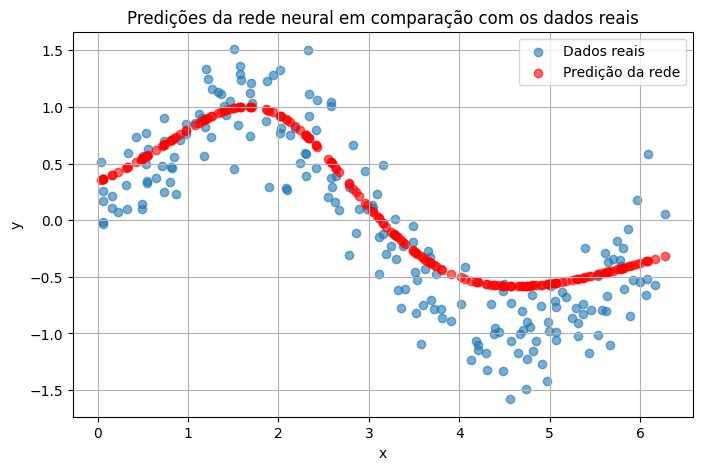
\includegraphics[width=\textwidth]{./0803_imgs/png-241110-154527304-12037654268696582542.png}
	%\legend{Fonte: Gerado peloComando da atividade}
	\end{minipage}
	\hfill
	\begin{minipage}{0.45\textwidth}
	\centering
	\caption{Treinando com 5000 épocas.}\label{tarefa02:5000:predicoes}
	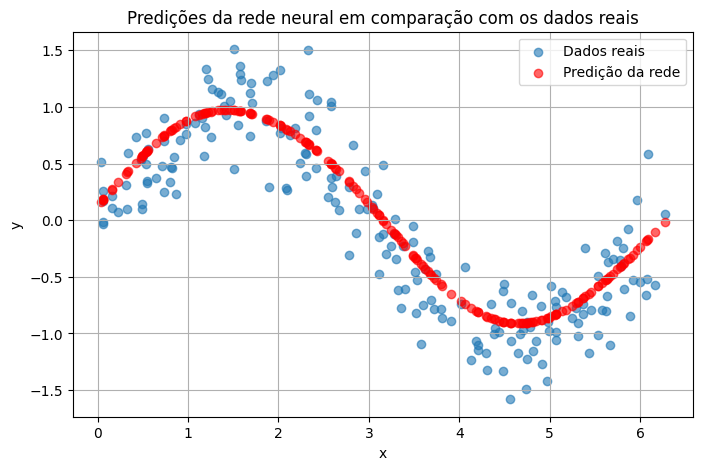
\includegraphics[width=\textwidth]{./0803_imgs/png-241110-154628196-17784737572676737911.png}
	%\legend{Fonte: \citeonline[p. 24]{araujo2012}}
	\end{minipage}
    \vspace{1Ex}
    \begin{minipage}{0.45\textwidth}
        \centering
        \caption{Treinando com 10000 épocas.} \label{tarefa02:10000:predicoes}
        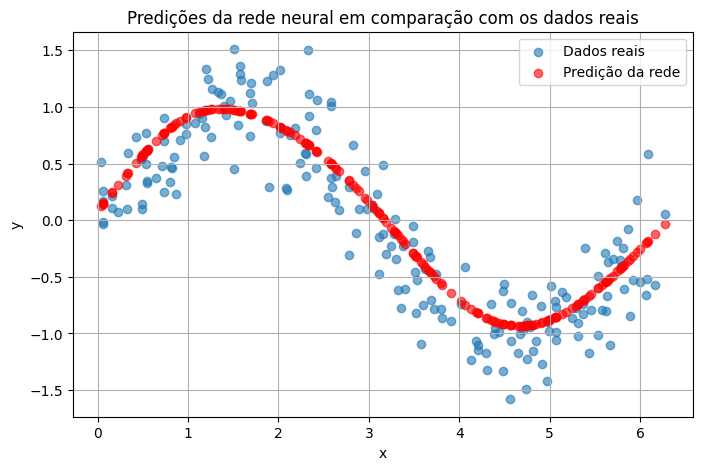
\includegraphics[width=\textwidth]{./0803_imgs/png-241110-154812342-18762265025268743.png}
        %\legend{Fonte: \citeonline[p. 24]{araujo2012}}
    \end{minipage}
\end{figure}
